%TODO: Die Schätzungen gehen nur von Veränderungen der verwendeten Menge bzgl.
%Transistoren aus. Wenn diese Menge nur ein Bruchteil ausmacht, dann hat auch
%die Verwendung einer Alternative kaum einen Einfluss. Das müssen wir noch
%irgendwie berücksichtigen.

\section{Wirtschaftlich}\label{sec:conflict}

Dieser Abschnitt beschreibt die wirtschaftliche Nachhaltigkeit von Tantal für alle abgehandelten Szenarien. Die Nachhaltigkeitsanalyse beschäftigt sich dabei mit dem globalen Effekt des Tantalabbaus.

\subsection{Indikatoren}

\paragraph{Preis}
Mittels Indikator ``Preis'' untersucht man, wie sich der Preis pro Kilo Tantal
in amerikanischen Dollars (USD) verändert. Eine Senkung wird als positiv bewertet, da die ICT-Branche von günstigeren Rohstoffpreisen profitiert. 

\paragraph{Arbeitsplätze}
Der Indikator ``Arbeitsplätze'' misst, wie die Produktion von Tantal die Anzahl
Arbeitsplätze beeinflusst. Die Qualität der Arbeitsplätze ist bei diesem Indikator kein Kriterium. Eine Erhöhung der Anzahl Arbeitsplätze wirkt sich positiv auf den Indikator aus.

\paragraph{Innovation}
Dieser Indikator misst, ob durch die Produktion von Tental neue Technologien
entstehen und ob diese nachhaltig die Marktentwicklung beeinflussen können. Steigt das Innovationspotential, steigt auch die Bewertung des Indikators.

\subsection{Bewertung}

\paragraph{2013}
Der \textbf{Preis} von Tantal pro Kilogramm betrug im Jahr 2006 USD 65.-, 2010 USD 121.- und 2013 USD 237.- ~\cite{tantal_price2}. 237 USD wird auf der Nachhaltigkeitsskala mit einer 5 als neutral eingestuft.

\begin{figure}[h]
\centering
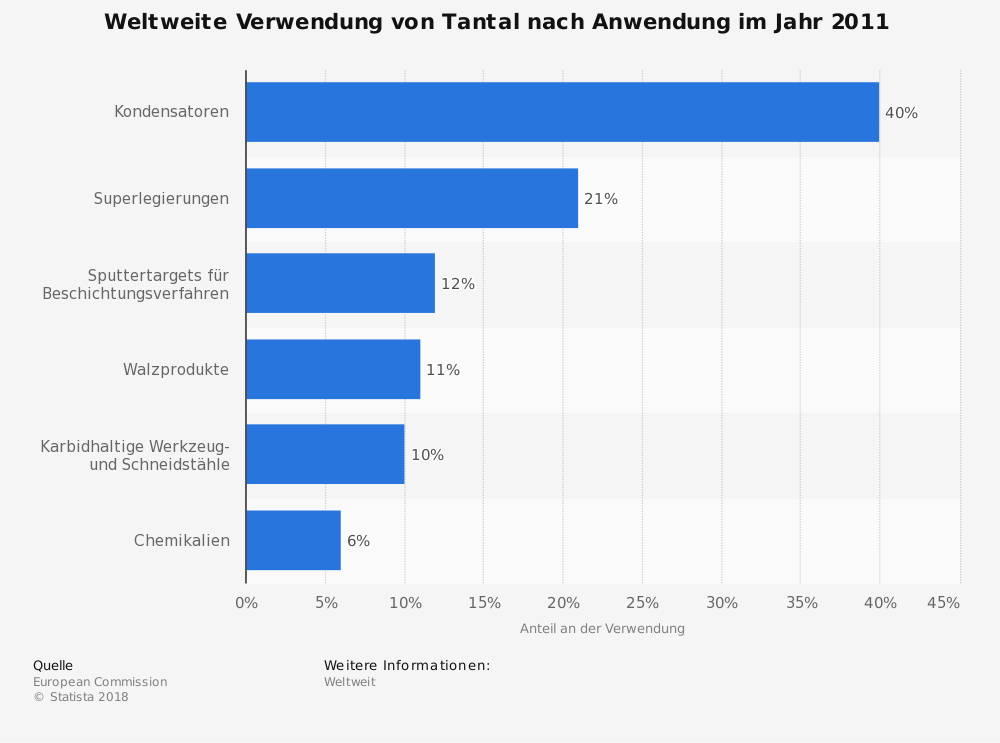
\includegraphics[width=0.8\textwidth]{tantal_usage_2011}
\caption{BGR. n.d. Weltweite Verwendung von Tantal nach Anwendung im Jahr 2011 ~\cite{tantal_usage}}
\label{}
\end{figure}

2013 wurden weltweit 1300 Tonnen Tantal in Bergwerken gefördert ~\cite{tantal_price2}. 2011 wurden 40\% des geförderteten Tantals für Kondensatoren verwendet. Bei gleichbleibender Verwendungsrate entspricht dies einer Fördermenge von 520 Tonnen im Jahr 2013.
% Hier Anzahl Jobs in Verhältnis zu Tonnen bringen. Dann kann man hochrechnen.
Da die Nachfrage von Tantal stetig steigt~\cite{tantal_price2}, Müssen auch mehr Arbeitskräfte angestellt werden. Somit wirkt sich der Tantalabbau positiv auf die Nachhaltigkeit der Anzahl \textbf{Arbeitsplätze} aus und erhält eine 6 auf der Nachhaltigkeitsskala.

Tantal ist ein essentieller Bestandteil von Transistoren, welche in Mikroprozessoren verwendet werden. Mikroprozessoren finden Verwendung in Computern und Maschinensteuerungen. Diese Geräte haben die Welt grundsätzlich verändert und erlauben der Menschheit effizienter zu arbeiten. Die Bewertung fällt für den Indikator \textbf{Innovation} mit 7 sehr positiv aus.

\paragraph{2035 bei anhaltendem Trend}
% Preis extrapolieren?
Bei steigender Nachfrage bezüglich Tantal wird der \textbf{Preis} ebenfalls weiterhin steigen. Man kann keine genauen Aussagen zum effektiven Preis machen. Da dieser aber bereits von 2006 bis 2013 um 364.62\% gestiegen ist~\cite{tantal_price2}, geht man davon aus, dass die Zunahme weiterhin bestehen bleibt. Der Preis erhält deswegen eine extrem negative Bewertung, was einer 1 entspricht.

Die Anzahl \textbf{Arbeitsplätze} werden ebenfalls von der steigenden Nachfrage beeinflusst. Bis 2035 ist damit zu rechnen, dass sich die Nachfrage von Tantal verdoppelt. Damit keine Engpässe entstehen, müssen neue Minen eröffnet und mehr Arbeitsplätze geschafen werden. Bereits im Jahr 2018 starten neue Minen in Australien den Abbau von Tantal.~\cite{new_mine_aus} Diese extrem positive Entwicklung führt zu einer 8 auf der Nachhaltigkeitsskala.

% sehr komische Annahme
Ein anhaltender Trend bedeutet, dass sich bezüglich Innovation nur wenig bis gar nichts verändert. Da immer noch Kondensatoren aus Tantal hergestellt werden und auch sonst keine grossen Veränderungen zu erwarten sind, wird die Innovation leicht schlechter mit einer 6 bewertet.

\paragraph{2035 mit Kondensatorenalternative}
% TODO: viel zu viele passive Sätze...
Obwohl eine Alternative für die Kondensatoren eine Entlastung des Tantalbedarfs in der ICT-Branche bedeutet, werden weiterhin andere Industrie auf Tantal angewiesen sein. Angenomen, der Anteil von 40\% der Tantalproduktion, welche für Kondensatoren verwendet werden, fällt weg, dann müssen trotzdem noch 305 Tonnen mehr als im Jahr 2013 gefördert werden.~\cite{tantal_price2} Der \textbf{Preis} wird somit immernoch leicht steigen und wird deshalb mit einer 4 auf der Nachhaltigkeitsskala bewertet.
% Bedarf 2035 sind 1070t für Kondensatoren, 1070/0.4*0.6 = 1605t für alles andere, heutiger Bedarf 1300t, Differenz ist 305t

Da die Nachfrage im Alternativszenario nicht so drastisch steigt, wie in der Prognose, muss die Fördermenge dennoch gesteigert werden. Dies wird zu mehr \textbf{Arbeitsplätzen} führen. Der Nachhaltigkeitsindex erhält eine 7.

% macht das irgendwie sinn?
Eine Technologie, die aus Tantal bestehnde Kondensatoren ablöst, ist innovativ und nachhaltig. Der Tantalabbau selbst besteht zwar immer noch, aber auf die Innovation hat sich dies positiv ausgewirkt und wird höher als zuvor mit einer 8 bewertet.

\begin{table}[h]
  \centering
  \begin{tabular}{l|ccc}            & \textbf{2013} & \textbf{2035} & \textbf{2035 mit Annahme}
    \\ \hline Preis                 & 5             & 1             & 4
    \\ Arbeitsplätze                & 6             & 8             & 7
    \\ Innovation                   & 7             & 6             & 8
    \\ \hline \textbf{Endbewertung} & 6             & 5             & 6\(\frac{1}{3}\)
  \end{tabular}
  \caption{Resultat wirtschaftliche Analyse}
\end{table}
